\chapter{Patterns of premature fruit drop in tropical forest plants}

% \setcounter{page}{1} 
% \pagestyle{myheadings}
% \markboth{}{}\markright{} \rhead{\thepage} \setcounter{page}{1}
% \pagestyle{myheadings} \pagenumbering{arabic} \rhead{\thepage}
\section{Introduction}
Seed production is a critical element in the life cycle of a plant, giving rise to the next generation and thereby mediating population- and community- level dynamics (\cite{clarkArePlantPopulations2007a, maronHerbivoryEffectsPlant2006, turnbullArePlantPopulations2000, greenNonrandomDiversifyingProcesses2014}). Mortality events that happen in early life (from seed to seedling) can be a bottleneck for the recruitment of individuals to a population, with sometimes disproportionate effects on community composition (\cite{roughgardenRecruitmentDynamicsComplex1988}). This is particularly evident in plant communities, where seed availability can be the limiting factor determining plant population abundance and distribution (\cite{jamesDemographicProcessesLimiting2011,fennerEcologySeeds2005,rotherDemographicBottlenecksTropical2013}). A number of processes contribute to the success or failure of a developing seed, including nutrient availability, microclimatic conditions and the interactions between the plant and other organisms. For plant species relying on biotic pollination, visits from pollinators are crucial for reproductive success, often manifesting as a direct positive correlation between pollinator visitation rate and seed set (\cite{karronMultiplePollinatorVisits2006, steffan-dewenterPollinationSeedSet2001}). Following successful pollination, the developing seed might be a target for a range of enemies, including pre-dispersal insect seed predators, with deleterious effects on fitness. \\

While the importance of natural enemies of seeds and seedlings in the ecology of tropical forests has received much attention since Janzen’s (1970) and Connell’s (1971) seminal papers on the role of natural enemies in tropical forests (\cite{harmsPervasiveDensitydependentRecruitment2000, bagchiPathogensInsectHerbivores2014}), the bulk of research has focused on natural enemies attacking seeds or young seedlings after their dispersal from the mother plant (\cite{comitaTestingPredictionsJanzenConnell2014, hollEffectsSpeciesHabitat1997, leviTropicalForestsCan2019}). Although pre-dispersal seed mortality has been highlighted as a potentially important source of mortality and facilitator of high local plant diversity in tropical forests (\cite{ janzenHerbivoresNumberTree1970}), the fate of the plant’s progeny in the period prior to seed dispersal – as the fruit is developing – is relatively understudied in tropical forests (but see \cite{jonesDensitydependentPredispersalSeed2010}).\\

A commonly observed phenomenon in plants – including rainforest trees (SG., pers. obs.) – is that some fruits are prematurely abscised, i.e. drop from the mother plant prior to having completed their development. The ecological and agricultural research literature reports a number of causes of premature fruit drop (Table \ref{tab:causes}). For example, biotic and abiotic factors can contribute to changes in resource availability, triggering an individual to drop fruit which is unlikely to reach maturity and thereby minimising cost to the parent plant (\cite{stephensonFlowerFruitAbortion1981}). Damage can also lead to premature abscission, often through seed/fruit predation or pathogenic attack. Regardless of the exact mechanism causing premature fruit abscission, the resulting seed mortality could – if it reduces the number of viable seeds produced by the plant – have important effects on plant population and community dynamics. To our knowledge, this is the first study investigating patterns of premature fruit abscission in a tropical plant community and could provide insights into the coexistence of high numbers of tree species in tropical forests. \\

In this study we investigated patterns of premature fruit fall in the woody plant community (trees, shrubs, lianas) of Barro Colorado Island, Panama. Taking advantage of a long-term multi-species data set on seed and fruit rain, we quantified levels of premature fruit abscission for 268 plant species. Our overall aim was to explore the community-level patterns of premature fruit abscission. More specifically:

\begin{enumerate}
\item To describe and quantify interspecific variation in fruit abscission rates
\item To test whether variation in fruit abscission rates can be explained by plant phylogeny and selected plant traits (Table \ref{tab:traits})
\item To test whether premature fruit abscission rates are highest in plant species known to be attacked by internally-feeding, pre-dispersal insect seed predators
\end{enumerate} 

We hypothesised that:
\begin{itemize}
\item Seed enemies are the cause of some premature fruit drop
\item Plant species with traits hypothesised to make them more prone to enemy attack (Table \ref{tab:traits}) will have higher rates of premature fruit abscission
\item Some traits are conserved among closely related plant species (Table \ref{tab:traits}), hence phylogeny may explain some of the variation between species 
\end{itemize} \\


\begin{sidewaystable}
\small
\begin{tabular}{|p{4cm}p{4cm}p{12cm}|}
\hline
        \textbf{Cause} &  & \textbf{e.g.} \\ \hline
        Resource limitation & Herbivory / Defoliation & \cite{cunninghamFruitSettingWatermelons1940,mehouachiDefoliationIncreasesFruit1995,yangBurstReactiveOxygen2015,jamesonResponsesIndividualPlants1963,janzenSeedingPatternsTropical1978,mcalisterResponseSoybeansLeaf1958,simmondsFurtherEffectsDefoliation1951,willsonAdaptiveDesignFloral1974} \\ \hline
         & Leaf shading & \cite{dashSevereShadingReduces2012,einhornABAShadingInduce2018,zhuAbscisicAcidEthylene2009,byersInfluenceLowLight1991,mayEffectShadingFruitfulness1963} \\ \hline
         & Nutrient depletion & \cite{bradburyComparativeStudyDeveloping1929,nightingaleEffectsNutrientConcentration1936,zhaoCottonGrowthPhysiological2003,bertaminiGrapevineGrowthPhysiological2005,martinez-alcantaraNitrogenuseEfficiencyYoung2012} \\ \hline
         & Frost & \cite{rodrigoSpringFrostsDeciduous2000,rodrigoSpringFrostDamage2006,addicottPhysiologyAbscission1955,addicottPhysiologicalEcologyAbscission1973,krugmanFreezingSpringTemperatures1966,tagliasacchiCytohistologicalCytochemicalFeatures2006,dorseyStudySterilityPlum1919} \\ \hline
         & Heat & \cite{zhouPhysiologicalResponseHeat2017,najeebEndogenousEthyleneConcentration2017} \\ \hline
         & Drought & \cite{reichardtPeptideSignalingDroughtinduced2020, udovenkoEffectDroughtOverheating1986,perez-perezResponseSweetOrange2008} \\ \hline
         & Leaf shading & \cite{dashSevereShadingReduces2012,einhornABAShadingInduce2018,zhuAbscisicAcidEthylene2009,byersInfluenceLowLight1991,mayEffectShadingFruitfulness1963} \\ \hline
        Damage to developing fruit & Seed predation & \cite{boucherEarlyDropNuts1979,dohanianControlFilbertWorm1944,lloydSexualStrategiesPlants1980,mattsonRoleInsectsDynamics1978,janzenSeedPredationAnimals1971,janzenSeedeatersVsSeed1969,janzenEscapeCassiaGrandis1971} \\ \hline
         & Fruit predation & \cite{planesWithintreeTemporalDistribution2014,bendaFruitAbscissionPhysalis2009,petzoldEffectHeliothisSubflexa2009, millerObservationsMelamphausFaber1932,phillipsImmatureNutfallCoconuts1940} \\ \hline
         & Pathogen attack & \cite{phillipsImmatureNutfallCoconuts1940,carterInjuriesPlantsCaused1939,akinsanmiFruitAbscissionMacadamia2016,teviotdaleAbscissionKernelQuality1997} \\ \hline
         & Genetic or developmental abnormalities & \cite{bradburyComparativeStudyDeveloping1929,krausSelfsterilityProblem1915,forinoEmbryosacsFrequencyOvules1987} \\ \hline
\end{tabular}
\caption{Causes of premature fruit drop}
\label{tab:causes}
\end{sidewaystable}
\\


\begin{sidewaystable}
\small
\begin{tabular}{|p{4cm}p{4cm}p{13cm}|}
\hline
        \textbf{Variable} & \textbf{Prediction} & \textbf{Hypothesis} \\ \hline
        Seed mass & Increased abscission with increased seed mass & Larger seeds are more valuable as a food source to potential seed predators (\cite{moegenburgSabalPalmettoSeed1996, fennerRelationshipCapitulumSize2002}). Additionally, large seeds might be exposed to predation from a wider range of seed predators (\cite{greigPredispersalSeedPredation1993, mucunguziBruchidsSurvivalAcacia1995}) and for a longer period of time (\cite{molesLatitudeSeedPredation2003}, but see \cite {molesSmallseededSpeciesHave2003}) \\ \hline
        abundance of plant conspecifics & increased abscission with increased abundance & Species with many conspecifics in the surrounding area are more prone to seed predator attack since the abundance of resources available to host-specific seed predators will be higher (\cite{janzenHostPlantsIslands1968}). However, predators may also become satiated when seeds are dense (\cite{burkeyTropicalTreeSpecies1994}). \\ \hline
        Overlap in fruit production by other species (CoFruit) & Increased abscission with increased overlap & Species fruiting at times of the year when few other species fruit are more apparent to enemies and prone to seed predator attack. Species which fruit in tandem with others, called masting, use this to their advantage (\cite{toyInterspecificFloweringPatterns1991, toyFruitingPhenologySurvival1992, kellyEvolutionaryEcologyMast1994}) \\ \hline
        Interannual variation in seed crop sizes & increased abscission with decreased variation & Species with temporally predictable fruiting patterns are more prone to seed predator attack since they provide a more stable resource seed predators (\cite{janzenSeedPredationAnimals1971,janzenWhyBamboosWait1976}) \\ \hline
        Endocarp investment (degree of investment in mechanical seed defences) & Increased abscission with decreased investment & Species that invest large amounts of resources in seed protection are less vulnerable to predation (\cite{benkmanImpactTreeSquirrels1995, rodgersonMechanicalDefenseSeeds1998,gathuaEffectsPrimatesSquirrels2000,kuprewiczMammalInsectPredation2010}) \\ \hline
        Average tree height & increased abscission with increased height & Taller species are more apparent to enemies (\cite{gripenbergHighlyResolvedFood2019, janzenHostPlantsIslands1968}) \\ \hline

\end{tabular}
\caption{Plant traits hypothesised to influence susceptibility to attack by pre-dispersal enemies}
\label{tab:traits}
\end{sidewaystable}


\section{Methods}
\emph{Study site}\\*
Barro Colorado Island (BCI; 9\degree9’N, 79\degree51’W), is a 16 km2 island situated in the Panama Canal, which supports semideciduous tropical forest with a 35m tall canopy. BCI became a reserve in 1923 and ecological studies have been carried out here for more than 100 years. The island is known for its 50 ha permanent forest dynamics plot – the first to be established within the CTFS-ForestGEO plot network in 1982 (\cite{anderson-teixeiraCTFSForestGEOWorldwideNetwork2015}). Within the 50-ha plot, all free-standing woody plants larger than 1 cm in diameter at breast height are mapped and measured at five-year intervals. The censuses have recorded 299 different tree species in the plot (\cite{ anderson-teixeiraCTFSForestGEOWorldwideNetwork2015}). Long-term studies of the forest dynamics plot at BCI have yielded considerable data on the spatial and temporal dynamics of tropical forests and led to many new insights into tropical forest ecology, including to species coexistence theory (e.g. \cite{conditBetaDiversityTropicalForest2002, comitaTestingPredictionsJanzenConnell2014, harmsPervasiveDensitydependentRecruitment2000}).\\

\emph{Seed Rain}\\*
Since 1987, weekly censuses of seed rain have been conducted within the 50-ha Forest Dynamics Plot as part of a research project coordinated by Dr S. J. Wright (Smithsonian Tropical Research Institute) (\cite{ wrightAnnualSpatialVariation2005}). 250 seed traps are set along 2.7 km of trails within the plot, at 13.5-m intervals on alternating sides of the trail at locations between 4 and 10 m from the trail so that distances between neighbouring traps average 18.9 ± 3.6 m (mean ± 1 SD). Each trap consists of a 0.8m tall PVC frame and 1mm mesh covering a 0.5m\textsuperscript{2} square of forest floor. In weekly censuses of the traps, seeds, fruits and flowers are identified to species and counted. Fruits are categorised as mature (endosperm of seeds is filled) or immature (endosperm is not filled). In this study, only observations of fruits and seeds were used and species were limited to woody plant species (trees, lianas and shrubs). \\
Species-specific proportions of prematurely abscised seeds were calculated as abscised seeds as a proportion of total seeds weighted by year.

\[proportion abscised = \frac{abscised seeds}{viable seeds + abscised seeds}\ \]
  

Where;\\*
Abscised seeds = immature fruits × mean number of seeds per fruit\\*
Viable seeds = single diaspores + (mature fruits × mean number of seeds per fruit)\\*

For each species, we first calculated yearly premature fruit abscission rates by pooling the data from all individual seed traps in which the species occurred for each full calendar year in the data set (1987 to 2019; n = 23 years). We used the species-specific averages of these values in further analyses.\\

Of the 311 woody plant species in the full seed rain dataset, 268 had data available regarding the typical number of seeds per fruit (required to calculate the numbers of abscised and viable seeds). To ensure a reasonable sample size of fruits, species were excluded from the analysis if total seeds (abscised + viable) across all years was lower than 50, leaving 201 species in the dataset (Table \ref{tab:summary}).\\

\begin{table}
    \centering
    \caption{Summary of seed rain dataset}
    \begin{tabular}{|l|l|l|l|l|l|}
    \hline
        Lifeform &     Mature fruit &      Single diaspores &     Immature fruit &      Species &         Families \\ \hline
        Liana &                83,785  &                39,052  &                74,917  &     55  &                         18  \\ \hline
        Midstory &                49,604  &                37,480  &              105,284  &      21  &                         16  \\ \hline
        Shrub &                   4,491  &                54,425  &                   8,084  &     20  &                         11  \\ \hline
        Tree &              312,650  &              601,120  &              386,617  &               66  &                         29  \\ \hline
        Understory &              184,530  &              363,429  &              101,473  &      39  &                         19  \\ \hline
         Total &              635,060  &          1,095,506  &              676,375  &            201  &                         93  \\ \hline
    \end{tabular}
    \label{tab:summary}
\end{table}

\emph{Plant phylogeny and trait data}\\*
Data on traits listed in Table \ref{tab:traits} was obtained from a variety of sources as detailed in \cite{gripenbergHighlyResolvedFood2019} and \cite{wrightFunctionalTraitsGrowth2010}. Information on the presence and abundance of seed predators on individual plant species was obtained from a study by \cite{gripenbergHighlyResolvedFood2019} in which insects were reared from seeds or fruits collected on BCI. A phylogeny which included 197 of the plant species in our data set was provided by David Erickson (Smithsonian Institution).  The phylogeny was constructed following methods in \cite{kressPlantDNABarcodes2009}. \\

\emph{Analysis}\\*
To investigate the relationships between premature fruit abscission and our selected plant traits (Table \ref{tab:traits}) I calculated Spearman’s rank correlation coefficients and visualised these relationships in scatter plots. Co-variance of traits was assessed with a correlation matrix using the R package ggcorrplot.\\

To explore how well shared phylogenetic ancestry can account for similarities in premature fruit abscission among species within the community, I estimated the phylogenetic signal (the tendency for related species to be more similar than species drawn at random from the phylogenetic tree) in the proportion of fruits prematurely abscised using the phylosig function in the package phytools (\cite{revellPhytoolsPhylogeneticTools2020}). The phylogenetic signal was assessed using Pagel’s \textlambda, which varies from 0 (where phylogenetic and trait similarity are totally independent) to 1 (where the traits are completely explained by shared ancestry). The contMap function in the R package phytools (\cite{revellPhytoolsPhylogeneticTools2020}) was used to visualise phylogenetic signal as a continuous trait mapped onto the phylogenetic tree. I then explored the relationship between selected plant traits (Table \ref{tab:traits}) and the average proportion of seeds abscised, using linear regressions accounting for phylogenetic non-independence between related species, with the function pgls in the R package caper (\cite{ormeCaperComparativeAnalyses2018}). I compared these phylogenetically ‘corrected’ regressions to ordinary least squares (OLS) regressions generated using the lm function. I visualised the relationships between premature fruit abscissison rates and individual traits using scatter plots overlaid with lines describing the outputs of both the lm and pgls models.\\

The difference in proportion of abscised seeds between plant species that were known to be attacked by insect seed predators and those that were not, was assessed using a two-sample test and visualised using boxplots. The relationship between community-level patterns of insect seed predation and premature fruit abscission was described by fitting a general linear model with binomial logistic regression using the glm function. The cbind function was used to give higher weighting to species with a greater sample size of seeds (i.e. a higher number of total seeds). The fitted values from the model were overlaid onto a scatter plot of the data to assess goodness of fit.\\

\section{Results}
Our results indicate that premature fruit abscission in the forest dynamics plot is common. Of the 1,311,706 fruits collected in the seed rain traps across all years and plant species, 676,533 were immature (52\%). Taking into account single diaspores collected in the traps and the mean number of seeds per fruit for each species, of 8,996,317 total seeds sampled, 3,270,289 were abscised prematurely (36\%). No prematurely abscised fruits were collected for 30 species (Figure \ref{fig:hist}), the remaining 171 species all abscised some seeds with 49 abscising more than 50\% of total seeds on average across the 32-year study period.\\

\begin{figure}[!h]
\centering
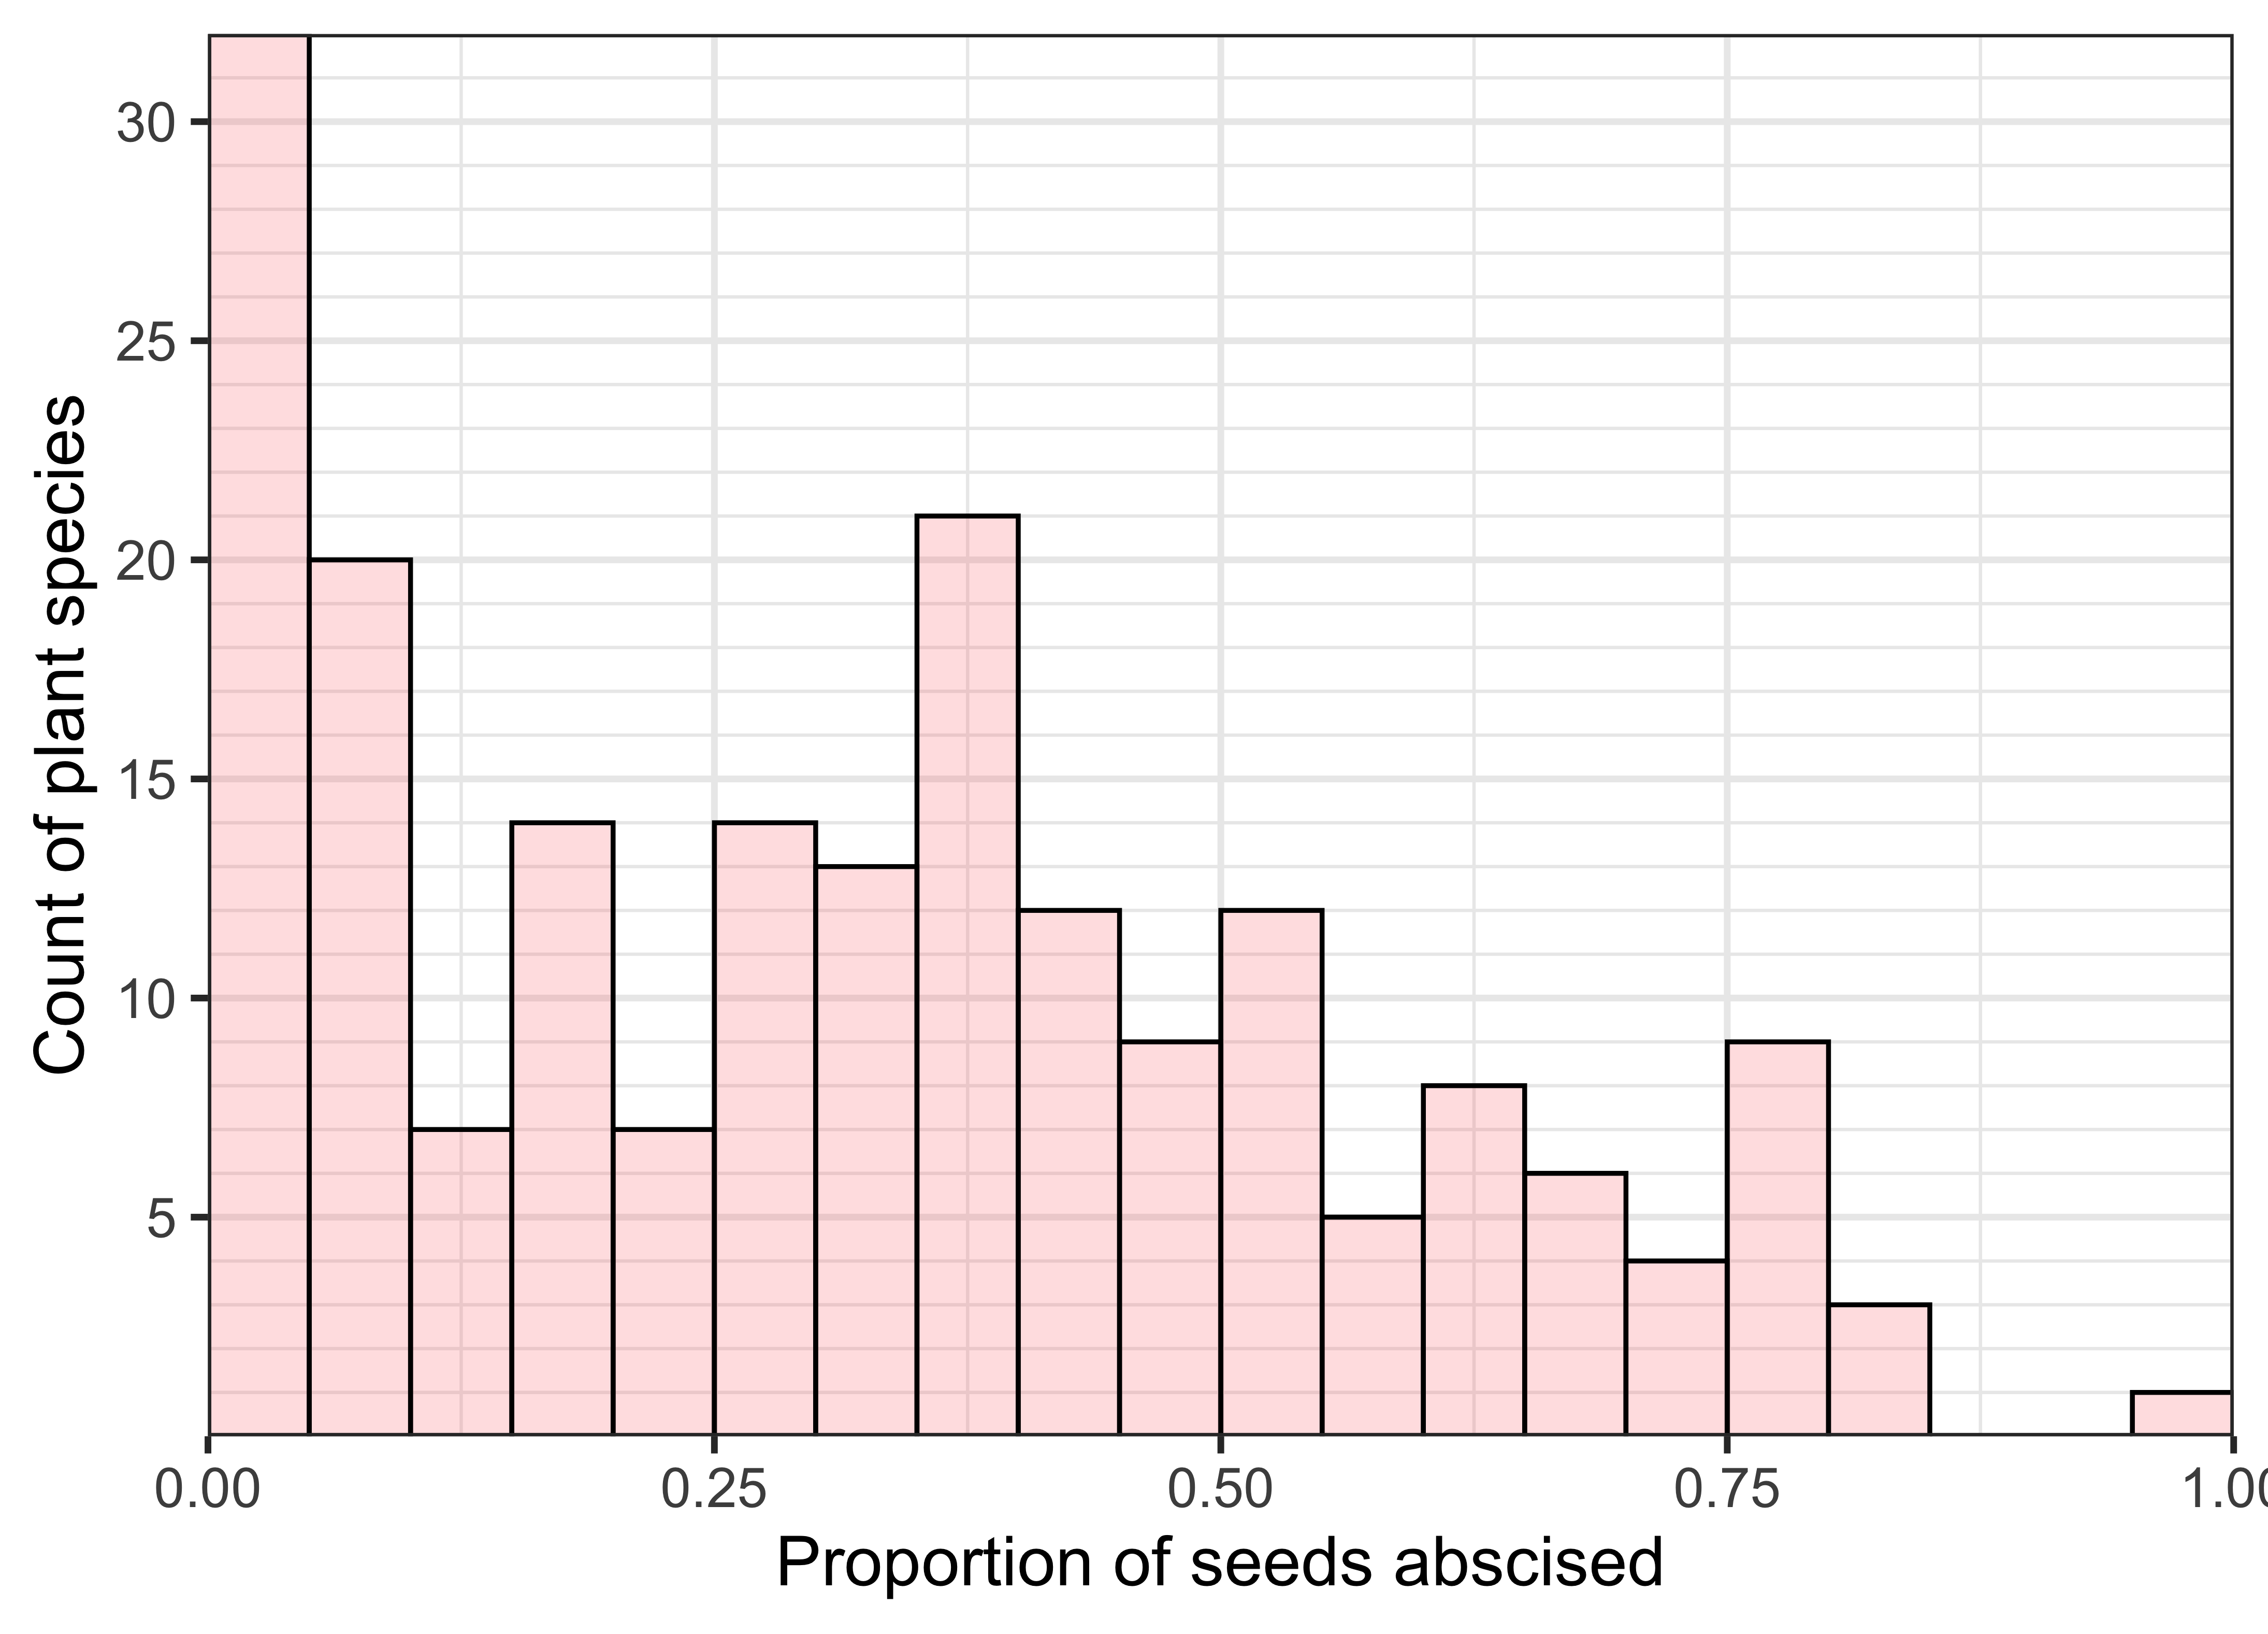
\includegraphics[width=10cm]{overallHist.png}
\caption{Histogram showing the frequency distribution of proportion of abscised seeds across all species}
\label{fig:hist}
\end{figure}

Of the selected plant traits, average tree height showed the strongest linear correlation with the proportion of abscised seeds (Figure \ref{fig:corr}; Spearman’s rho = 0.36, p = \textless 0.05), however, the linear correlations did not appear to fit well to the data. The correlations between some of the studied traits were relatively strong. For example, the overlap in fruit production correlated negatively with interannual crop size variation (Figure \ref{fig:corrmat}; rho = -0.54, p = \textless 0.05) and positively with average tree height (Figure \ref{fig:corrmat}; rho = 0.43, p= \textless 0.05).\\

\begin{figure}[!h]
\centering
\includegraphics[width=10cm]{traitsScatter.png}
\caption{Spearman’s rank correlations between proportion of abscised seeds and plant traits. Shaded areas show 95\% confidence intervals.}
\label{fig:corr}
\end{figure}

\begin{figure}[!h]
\centering
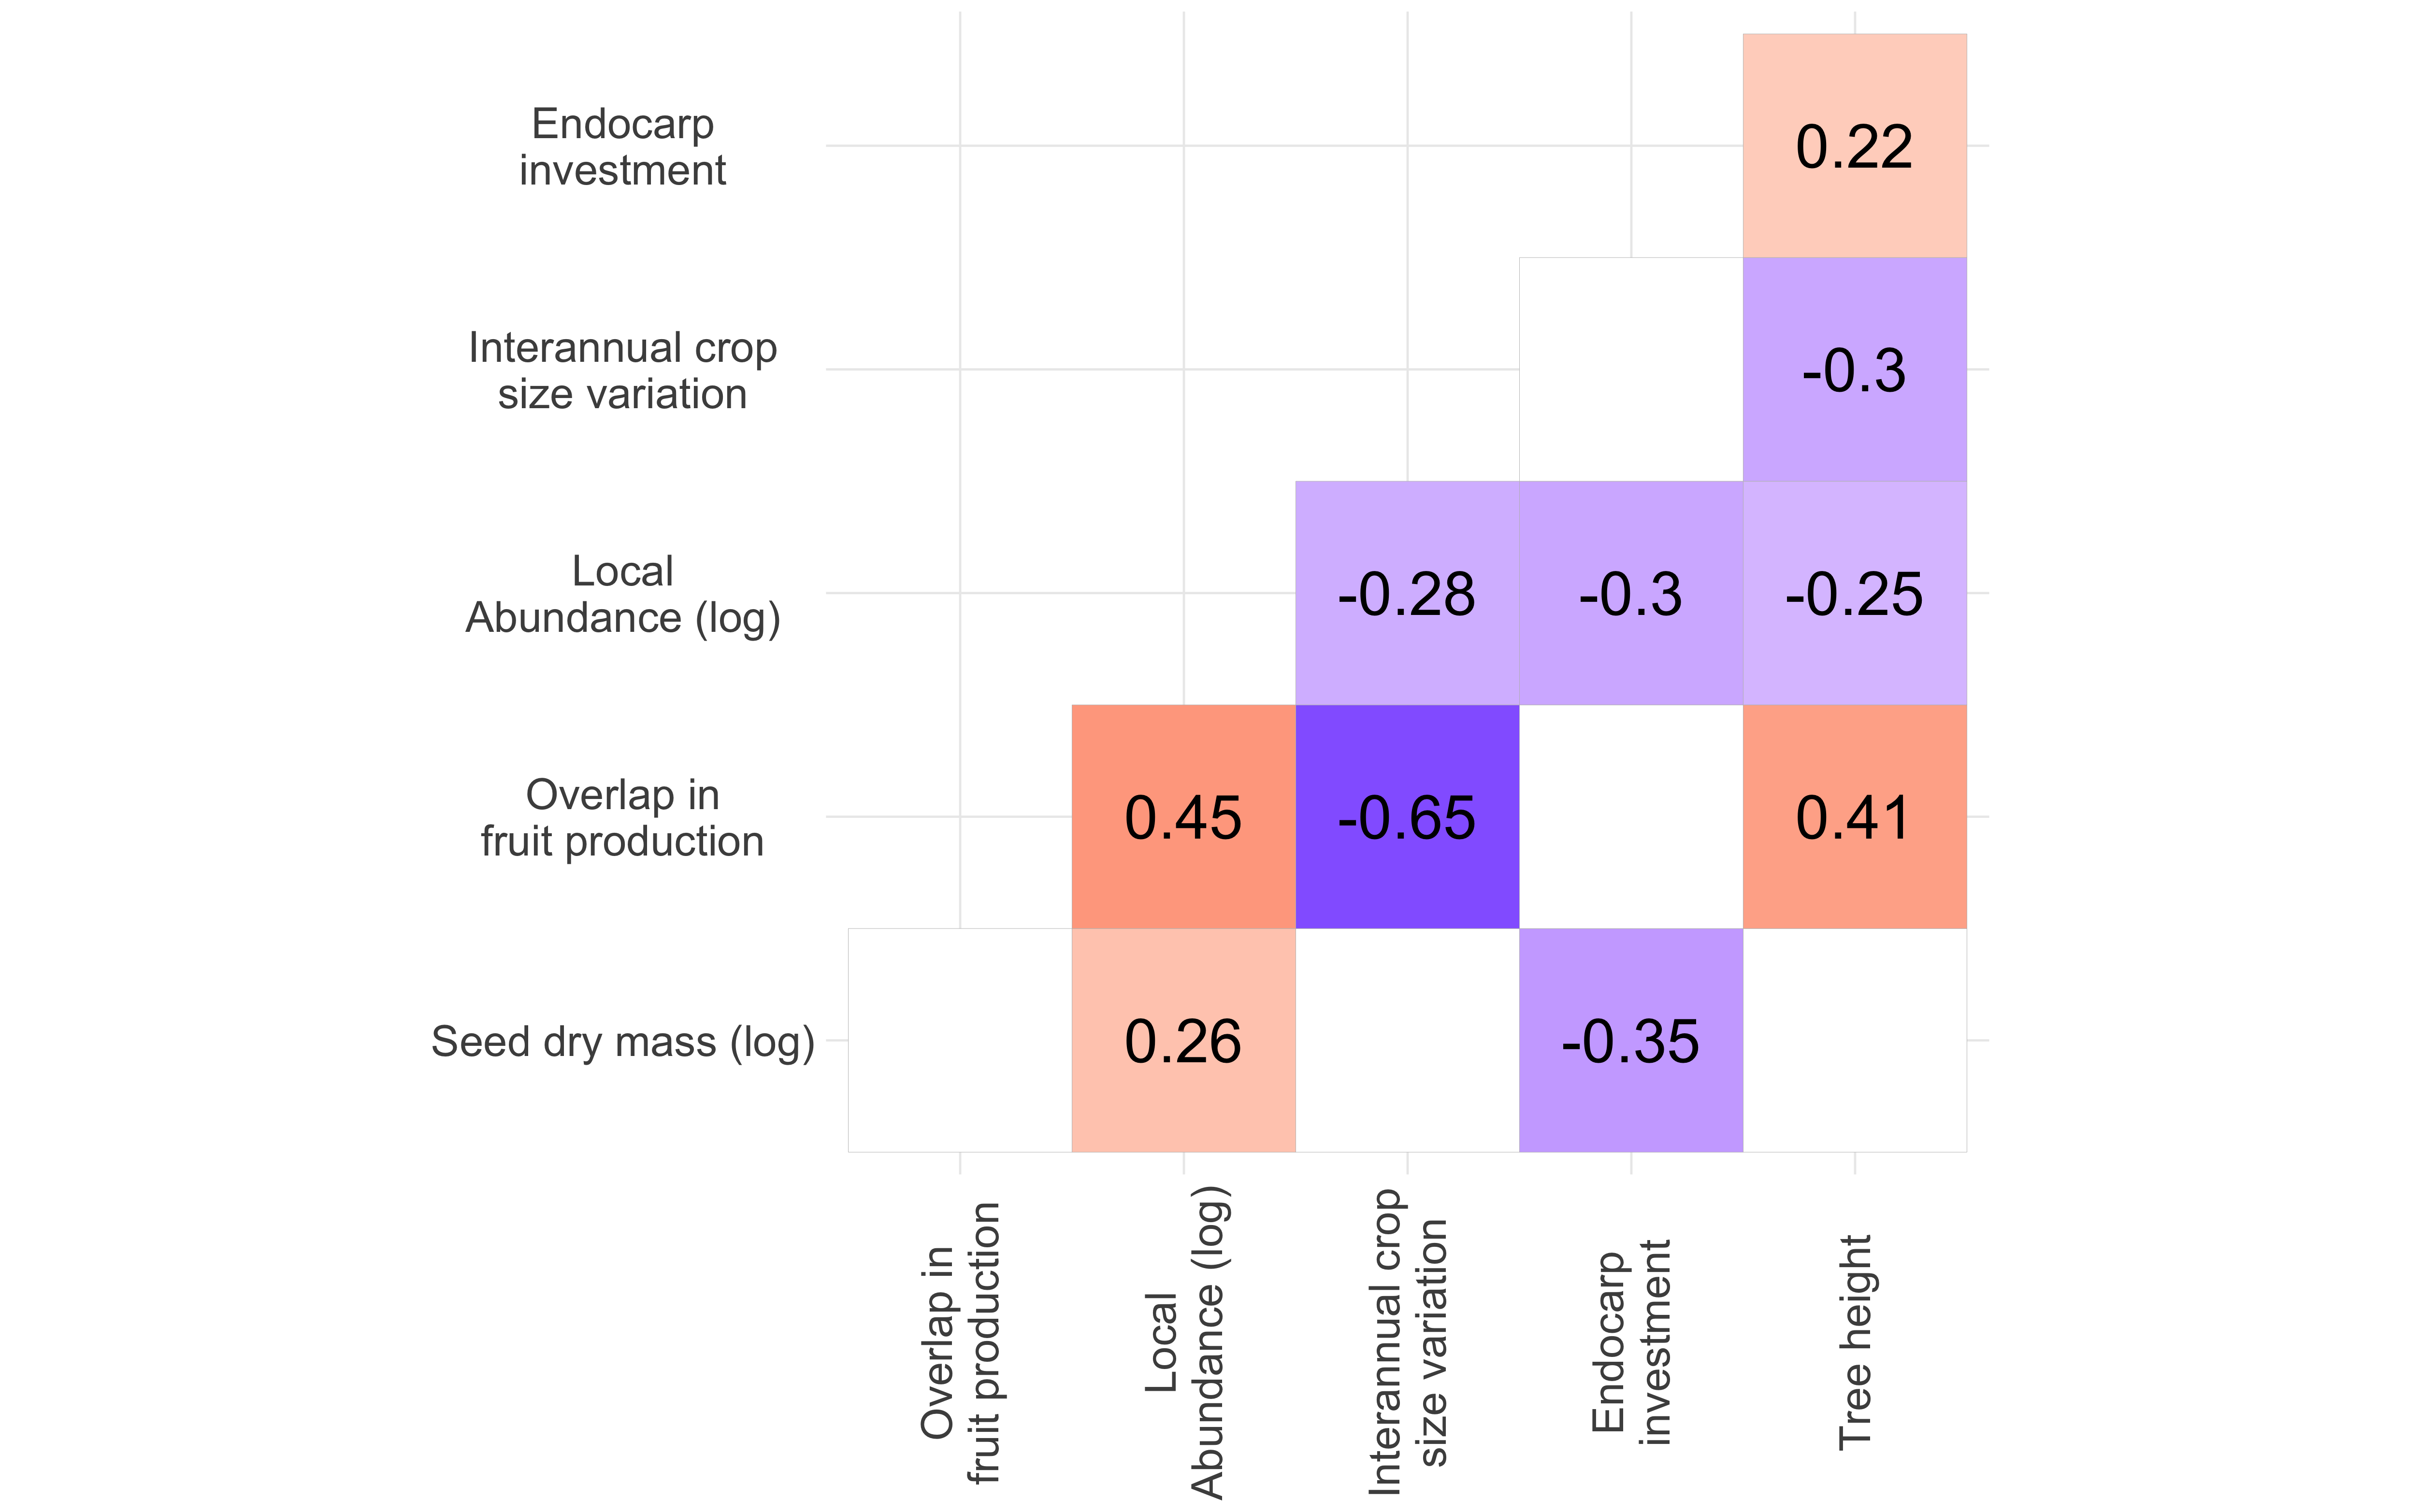
\includegraphics[width=10cm]{traitsCorr.png}
\caption{Correlations between plant traits. Numbers and colour show Spearman’s rank correlation coefficient, blank tiles indicate correlations for which p = \textless0.05}
\label{fig:corrmat}
\end{figure}

Phylogenetic models indicated phylogenetic non-independence in the relationships between premature fruit abscission and selected plant traits (Figure \ref{fig:phylomod}). Lambda was statistically significantly different from 0 in all models. However, the confidence intervals for the maximum likelihood lambda estimates were large indicating that we cannot be confident in the estimated value of lambda. Phylogenetic regression coefficients were also low suggesting that the studied plant traits are poor predictors of levels of premature fruit abscission (Table \ref{tab:phylomod}). 
The average proportion of seeds abscised was preserved phylogenetically (Figure \ref{fig:phylotree}; \textlambda = 0.33; p = \textless 0.001). Our results suggest that most species exhibit low or intermediate levels of premature fruit abscission (Figure \ref{fig:hist}), which is maintained evolutionarily (Figure \ref{fig:phylotree}). Only a few species abscise a large proportion of their seeds and this appears to show less phylogenetic signal; species with very high abscission rates are spread fairly evenly throughout the phylogenetic tree (Figure \ref{fig:phylotree}).\\

\begin{figure}[!h]
\centering
\includegraphics[width=10cm]{pgls.pdf}
\caption{Phylogenetic linear models of plant traits and premature fruit abscission. The red line is the phylogenetic linear model and the black is an OLS regression fitted to the data. Each point represents one species.}
\label{fig:phylomod}
\end{figure}


\begin{table}
\small
    \centering
    \caption{Model summary of phylogenetic linear models}
    \begin{tabular}{|p{3cm}|p{2cm}|p{2cm}|p{2cm}||p{2cm}|p{2cm}|}
    \hline
        \multirow{2}{*}{Plant trait} & \multicolumn{3}{l}{\textbf{Maximum likelihood \textlambda estimate }} & \multicolumn{2}{l}{\textbf{Phylogenetic linear model}} \\
        \cline{2-6}
        & \lambda & 95\% confidence intervals & p & Adjusted R-squared & p \\ \hline
        Local Abundance (n = 133) & 0.242 & 0.047, 0.483 & 0.002  & 0.047 & 0.006 \\ \hline
        Seed dry mass (n = 190) & 0.242 & 0.072, 0.487 & \textless0.001 & 0.053 & \textless0.001 \\ \hline
        Tree height (n = 137) & 0.255 & 0.030, 0.518 & 0.023 & 0.11 & \textless0.001 \\ \hline
        Interannual crop size variation (n = 159) & 0.22 & 0.059, 0.457 & 0.001 & 0.028 & 0.019 \\ \hline
        Overlap in fruit production (n = 184) & 0.344 & 0.159, 0.552 & \textless0.001 & 0.1 & \textless0.001 \\ \hline
        Endocarp investment (n = 185) & 0.288 & 0.103, 0.513 & \textless0.001 & 0.003 & 0.486 \\ \hline
    \end{tabular}
    \label{tab:phylomod}
\end{table}

\begin{figure}[!h]
\centering
\includegraphics[width=15cm]{ContMap.png}
\caption{Phylogenetic signal of premature fruit abscission for 197 species. Blue represents an average proportion of abscised seeds is equal to 1 and red is equal to 0. Phylogenetic signal of premature fruit abscission was estimated using Pagel’s lambda (\textlambda = 0.33; p = \textless0.001)}
\label{fig:phylotree}
\end{figure}

Species for which there was no incidence of seed predators had significantly lower levels of seed abscission (mean = 0.241), than those that did (mean = 0.388) (Figure \ref{fig:seedbox}; two sample t-test; p= \textless0.001). Seed predation rate only explained a small proportion of the variation in premature fruit abscission rates (Figure \ref{fig:seedscatter}; R = 0.07, p= \textless0.001). \\

\begin{figure}[!h]
\centering
\includegraphics[width=10cm]{predPres.png}
\caption{Premature fruit abscission and presence of seed predators. The proportion of seeds abscised plotted against presence of seed predator, presence is 0 where no seed predators were found in fruits of that plant species, presence is 1 where a seed predator was found. Panel (a) includes all insect seed predators, panel (b) shows the presence of insect orders Coleoptera, Hymenoptera and Lepidoptera independently. The average proportion of seeds abscised was significantly higher for plant species known to be attacked by insect seed predators (presence of seed predator = 1) (two sample t-test; p= \textless0.001).}
\label{fig:seedbox}
\end{figure}

\begin{figure}[!h]
\centering
\includegraphics[width=10cm]{glm.png}
\caption{Relationship between premature fruit abscission and rate of seed predation. Rate of seed predation is plotted against proportion of seeds abscised for each species in black. Red points represent fitted values from a generalized linear model.}
\label{fig:seedscatter}
\end{figure}

\section{Next steps}

\begin{itemize}
\item To expand generalised linear models of premature fruit abscission and rate of seed predation to include interactions of plant traits
\item To optimise lambda in phylogenetic linear models and include interactions with plant traits by removing the least significant terms from a full model (including all traits), in a step-by-step process
\end{itemize} \\